% the template is adapted from https://github.com/kourgeorge/arxiv-style

\documentclass{article}


\usepackage{arxiv}

\usepackage[utf8]{inputenc} % allow utf-8 input
\usepackage[T1]{fontenc}    % use 8-bit T1 fonts
\usepackage{hyperref}       % hyperlinks
\usepackage{url}            % simple URL typesetting
\usepackage{booktabs}       % professional-quality tables
\usepackage{amsfonts}       % blackboard math symbols
\usepackage{nicefrac}       % compact symbols for 1/2, etc.
\usepackage{microtype}      % microtypography
\usepackage{lipsum}		% Can be removed after putting your text content

\usepackage{tikz} 
\usetikzlibrary{matrix}


\title{Some not that novel approach to image processing using nonparametric statistic learned from course}

%\date{September 9, 1985}	% Here you can change the date presented in the paper title
%\date{} 					% Or removing it

\author{
  Zhuo Yueyi \\ %\thanks{Use footnote for providing further
    %information about author (webpage, alternative
    %address)---\emph{not} for acknowledging funding agencies.} \\
  Department of Computer Science and Engineering\\
  Nanjing University of Science and Technology\\
  \texttt{yiyuezhuo@gmail.com} \\
}

\begin{document}
\maketitle

\begin{abstract}
%\lipsum[1]
This is a class paper for nonparametric statistical. 
All of methods introduced by \cite{wasserman2006all} will get a example to show how it can be applied on
image processing problem.
\end{abstract}


% keywords can be removed
\keywords{Nonparametric statistic \and image processing }


\section{Introduction}
%\lipsum[2]
%\lipsum[3]




\section{Data of image processing}
%\label{sec:headings}
%\lipsum[4] See Section \ref{sec:headings}.

RGB image can seen as a 3 variable function $f(i,j,c)$, $i,j$ denote the location of image, $c$ denotes
channel. The function can be coded by three matrixes as shown in Fig~\ref{fig:fig1}.

\begin{figure}[htb]
  \centering
  \begin{tikzpicture}
      \node[inner sep=0pt] (toad_rgb) at (0,0)
      {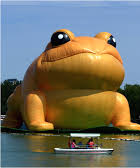
\includegraphics[width=.18\textwidth]{images/toad_rgb.png}};
      \node[inner sep=0pt] (toad_r) at (2.5,0)
      {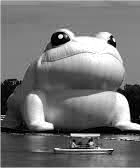
\includegraphics[width=.18\textwidth]{images/toad_r.png}};
      \node[inner sep=0pt] (toad_g) at (5,0)
      {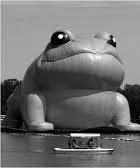
\includegraphics[width=.18\textwidth]{images/toad_g.png}};
      \node[inner sep=0pt] (toad_b) at (7.5,0)
      {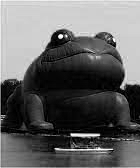
\includegraphics[width=.18\textwidth]{images/toad_b.png}};
      
      \draw [->] (toad_rgb.south) to [out=355, in=185] (toad_r.south);
      \draw [->] (toad_rgb.south) to [out=350, in=190] (toad_g.south);
      \draw [->] (toad_rgb.south) to [out=345, in=195] (toad_b.south);

      \draw [red] (7.5, 0.05) -- (7.6, 0.05) -- (7.6,-0.05) -- (7.5, -0.05) -- (7.5, 0.05);

      %\node (10.0,0.0) {$$\begin{bmatrix} 1 & 1 \\ 2 & 2 \end{bmatrix}$$};
      \matrix [matrix of nodes,row sep=-1ex, column sep=-1ex] (toad_mat) at (10.0, 0.0)
      {
          5 & 7 & 10 & 10 & 11 & 4 \\
          6 & 8 & 8 & 10 & 10 & 5 \\
          5 & 6 & 8 & 8 & 7 & 4 \\
          6 & 5 & 6 & 5 & 7 & 5 \\
          6 & 6 & 4 & 5 & 4 & 4 \\
          5 & 5 & 4 & 2 & 3 & 6  \\  };

      \draw [->] (7.6, 0.05) -- (toad_mat.north west);
      \draw [->] (7.6,-0.05) -- (toad_mat.south west);

      % draw matrix frame, how stupid I need to write it manually.
      \draw ([shift={(0.15, 0.0)}]toad_mat.north west) -- 
          ([shift={(0.05, 0.0)}]toad_mat.north west) --
          ([shift={(0.05, 0.0)}]toad_mat.south west) --
          ([shift={(0.15, 0.0)}]toad_mat.south west);

      \draw ([shift={(-0.15, 0.0)}]toad_mat.north east) -- 
          ([shift={(-0.05, 0.0)}]toad_mat.north east) --
          ([shift={(-0.05, 0.0)}]toad_mat.south east) --
          ([shift={(-0.15, 0.0)}]toad_mat.south east);

      \node at ([shift={(0.0, 0.2)}]toad_rgb.north) {RGB};
      \node at ([shift={(0.0, 0.2)}]toad_r.north) {R};
      \node at ([shift={(0.0, 0.2)}]toad_g.north) {G};
      \node at ([shift={(0.0, 0.2)}]toad_b.north) {B};
      \node at ([shift={(0.0, 0.2)}]toad_mat.north) {matrix of the crop};
      

      \draw[help lines] (0,0) grid (10,-10);
  \end{tikzpicture}
  \caption{Representation: Image as three matrix}
  \label{fig:fig1}
\end{figure}
 
\section{Jack}

\subsection{Headings: second level}
%\lipsum[5]
%\begin{equation}
%\xi _{ij}(t)=P(x_{t}=i,x_{t+1}=j|y,v,w;\theta)= {\frac {\alpha _{i}(t)a^{w_t}_{ij}\beta _{j}(t+1)b^{v_{t+1}}_{j}(y_{t+1})}{\sum _{i=1}^{N} \sum _{j=1}^{N} \alpha _{i}(t)a^{w_t}_{ij}\beta _{j}(t+1)b^{v_{t+1}}_{j}(y_{t+1})}}
%\end{equation}

\subsubsection{Headings: third level}
\lipsum[6]

\paragraph{Paragraph}
\lipsum[7]

\section{Examples of citations, figures, tables, references}
\label{sec:others}
\lipsum[8] \cite{kour2014real,kour2014fast} and see \cite{hadash2018estimate}.

The documentation for \verb+natbib+ may be found at
\begin{center}
  \url{http://mirrors.ctan.org/macros/latex/contrib/natbib/natnotes.pdf}
\end{center}
Of note is the command \verb+\citet+, which produces citations
appropriate for use in inline text.  For example,
\begin{verbatim}
   \citet{hasselmo} investigated\dots
\end{verbatim}
produces
\begin{quote}
  Hasselmo, et al.\ (1995) investigated\dots
\end{quote}

\begin{center}
  \url{https://www.ctan.org/pkg/booktabs}
\end{center}


\subsection{Figures}
\lipsum[10] 
See Figure \ref{fig:fig1}. Here is how you add footnotes. \footnote{Sample of the first footnote.}
\lipsum[11] 



\subsection{Tables}
\lipsum[12]
See awesome Table~\ref{tab:table}.

\begin{table}
 \caption{Sample table title}
  \centering
  \begin{tabular}{lll}
    \toprule
    \multicolumn{2}{c}{Part}                   \\
    \cmidrule(r){1-2}
    Name     & Description     & Size ($\mu$m) \\
    \midrule
    Dendrite & Input terminal  & $\sim$100     \\
    Axon     & Output terminal & $\sim$10      \\
    Soma     & Cell body       & up to $10^6$  \\
    \bottomrule
  \end{tabular}
  \label{tab:table}
\end{table}

\subsection{Lists}
\begin{itemize}
\item Item 1 Item 2
\item Item 3 Item 4
\item Item 5 Item 6
\end{itemize}


\bibliographystyle{unsrt}  
\bibliography{references}  %%% Remove comment to use the external .bib file (using bibtex).
%%% and comment out the ``the bibliography'' section.


\end{document}
